% ŠABLONA PRO PSANÍ ZÁVĚREČNÉ STUDIJNÍ PRÁCE
%%%%%%%%%%%%%%%%%%%%%%%%%%%%%%%%%%%%%%%%%%%%
% Autor: Jakub Dokulil (kubadokulil99@gmail.com)
% Tato šablona byla vytvořena tak, aby pomocí ní mohli v systému LaTeX soutěžící sázet své práce a zároveň odpovídala požadavkům na formátování vyplývajícím z wordové šablony umístěné na webu soc.cz.
%
\documentclass[12pt, a4paper,
%oneside,      %% -- odkomentujte, pokud chcete svou práci mít pouze jednostrannou, mezera pro hřbet pak automaticky bude pouze na levé straně
twoside,        %% -- pro oboustranné práce, mezera pro hřbet následně střídá strany.
openright
]{report}

%% Nutné balíčky a nastavení
%%%%%%%%%%%%%%%%%%%%%%%%%%%%





%% Proměnné
\newcommand\obor{INFORMAČNÍ TECHNOLOGIE} %% -- napiš číslo a název tvého oboru
\newcommand\kodOboru{18-20-M/01} %% -- napiš číslo a název tvého oboru
\newcommand\zamereni{se zaměřením na počítačové sítě a programování} %% -- napiš číslo a název tvého oboru
\newcommand\skola{Střední škola průmyslová a umělecká, Opava} %% vyplň název školy
\newcommand\trida{IT4} %% vyplň jméno svého konzultanta
\newcommand\jmenoAutora{Sofja Klopcová}  %% vyplň své jméno
\newcommand\skolniRok{2023/24} %% vyplň rok
\newcommand\datumOdevzdani{1. 1. 2024} %% vyplň rok
\newcommand\nazevPrace{Robotické rameno pohybující se pomocí gest} %% vyplň název své práce
\let\oldchapter\chapter
\renewcommand{\chapter}{
	\clearpage
	\pagestyle{fancy}
	\oldchapter
}



\title{\nazevPrace} %% -- Název tvé práce
\author{\jmenoAutora} %% -- tvé jméno
\date{\datumOdevzdani} %% -- rok, kdy píšeš SOČku

\usepackage[top=2cm, bottom=2.5cm, left=3.5cm, right=2cm]{geometry} %% nastaví okraje, left -- vnitřní okraj, right -- vnější okraj

\usepackage[czech]{babel} %% balík babel pro sazbu v češtině
\usepackage[utf8]{inputenc} %% balíky pro kódování textu
\usepackage[T1]{fontenc}
%\usepackage{cmap} %% balíček zajišťující, že vytvořené PDF bude prohledávatelné a kopírovatelné

\usepackage{graphicx} %% balík pro vkládání obrázků

\usepackage{subcaption} %% balíček pro vkládání podobrázků

\usepackage{hyperref} %% balíček, který v PDF vytváří odkazy

\linespread{1.25} %% řádkování
\setlength{\parskip}{0.5em} %% odsazení mezi odstavci


\usepackage[pagestyles]{titlesec} %% balíček pro úpravu stylu kapitol a sekcí
\titleformat{\chapter}[block]{\scshape\bfseries\LARGE}{\thechapter}{10pt}{\vspace{0pt}}[\vspace{-22pt}]
\titleformat{\section}[block]{\scshape\bfseries\Large}{\thesection}{10pt}{\vspace{0pt}}
\titleformat{\subsection}[block]{\bfseries\large}{\thesubsection}{10pt}{\vspace{0pt}}


\usepackage{tocloft} % Balíček umožní přizpůsobit vzhled tabulky obsahu
\setlength{\cftbeforechapskip}{0pt}  % Menší rozestup pro kapitoly
\setlength{\cftbeforesecskip}{0pt}   % Menší rozestup pro sekce

\setcounter{secnumdepth}{2}
\setcounter{tocdepth}{1}
\usepackage{fancyhdr}
\pagestyle{fancy}
\renewcommand{\headrulewidth}{0.025pt}

\usepackage{booktabs}

\usepackage{url}

%% Balíčky co se můžou hodit :) 
%%%%%%%%%%%%%%%%%%%%%%%%%%%%%%%

\usepackage{pdfpages} %% Balíček umožňující vkládat stránky z PDF souborů, 

\usepackage{upgreek} %% Balíček pro sazbu stojatých řeckých písmen, třeba u jednotky mikrometr. Například stojaté mí: \upmu, stojaté pí: \uppi

\usepackage{amsmath}    %% Balíčky amsmath a amsfonts 
\usepackage{amsfonts}   %% pro sazbu matematických symbolů
\usepackage{esint}     %% pro sazbu různých integrálů (např \oiint)
\usepackage{mathrsfs}
\usepackage{helvet} % Helvet font
\usepackage{mathptmx} % Times New Roman
\usepackage{Oswald} % Oswald font


%% makra pro sazbu matematiky
\newcommand{\dif}{\mathrm{d}} %% makro pro sazbu diferenciálu, místo toho
%% abych musel psát '\mathrm{d}' mi stačí napsat '\dif' což je mnohem 
%% kratší a mohu si tak usnadnit práci

\usepackage{listings}
\usepackage{xcolor}

\renewcommand{\lstlistingname}{Kód}% Listing -> Algorithm
\renewcommand{\lstlistlistingname}{Seznam programových kódů}% List of Listings -> List of Algorithms

%% Definice 
\lstdefinelanguage{JavaScript}{
	morekeywords=[1]{break, continue, delete, else, for, function, if, in,
		new, return, this, typeof, var, void, while, with},
	% Literals, primitive types, and reference types.
	morekeywords=[2]{false, null, true, boolean, number, undefined,
		Array, Boolean, Date, Math, Number, String, Object},
	% Built-ins.
	morekeywords=[3]{eval, parseInt, parseFloat, escape, unescape},
	sensitive,
	morecomment=[s]{/*}{*/},
	morecomment=[l]//,
	morecomment=[s]{/**}{*/}, % JavaDoc style comments
	morestring=[b]',
	morestring=[b]"
}[keywords, comments, strings]


\lstdefinelanguage[ECMAScript2015]{JavaScript}[]{JavaScript}{
	morekeywords=[1]{await, async, case, catch, class, const, default, do,
		enum, export, extends, finally, from, implements, import, instanceof,
		let, static, super, switch, throw, try},
	morestring=[b]` % Interpolation strings.
}

\lstalias[]{ES6}[ECMAScript2015]{JavaScript}

% Nastavení barev
% Requires package: color.
\definecolor{mediumgray}{rgb}{0.3, 0.4, 0.4}
\definecolor{mediumblue}{rgb}{0.0, 0.0, 0.8}
\definecolor{forestgreen}{rgb}{0.13, 0.55, 0.13}
\definecolor{darkviolet}{rgb}{0.58, 0.0, 0.83}
\definecolor{royalblue}{rgb}{0.25, 0.41, 0.88}
\definecolor{crimson}{rgb}{0.86, 0.8, 0.24}

% Nastavení pro Python
\lstdefinestyle{Python}{
	language=Python,
	backgroundcolor=\color{white},
	basicstyle=\ttfamily,
	breakatwhitespace=false,
	breaklines=false,
	captionpos=b,
	columns=fullflexible,
	commentstyle=\color{mediumgray}\upshape,
	emph={},
	emphstyle=\color{crimson},
	extendedchars=true,  % requires inputenc
	fontadjust=true,
	frame=single,
	identifierstyle=\color{black},
	keepspaces=true,
	keywordstyle=\color{mediumblue},
	keywordstyle={[2]\color{darkviolet}},
	keywordstyle={[3]\color{royalblue}},
	literate=%
	{á}{{\'a}}1 {č}{{\v{c}}}1 {ď}{{\v{d}}}1 {é}{{\'e}}1 {ě}{{\v{e}}}1
	{í}{{\'i}}1 {ň}{{\v{n}}}1 {ó}{{\'o}}1 {ř}{{\v{r}}}1 {š}{{\v{s}}}1
	{ť}{{\v{t}}}1 {ú}{{\'u}}1 {ů}{{\r{u}}}1 {ý}{{\'y}}1 {ž}{{\v{z}}}1,		
	numbers=left,
	numbersep=5pt,
	numberstyle=\tiny\color{black},
	rulecolor=\color{black},
	showlines=true,
	showspaces=false,
	showstringspaces=false,
	showtabs=false,
	stringstyle=\color{forestgreen},
	tabsize=2,
	title=\lstname,
	upquote=true  % requires textcomp	
}


\lstdefinestyle{JSES6Base}{
	backgroundcolor=\color{white},
	basicstyle=\ttfamily,
	breakatwhitespace=false,
	breaklines=false,
	captionpos=b,
	columns=fullflexible,
	commentstyle=\color{mediumgray}\upshape,
	emph={},
	emphstyle=\color{crimson},
	extendedchars=true,  % requires inputenc
	fontadjust=true,
	frame=single,
	identifierstyle=\color{black},
	keepspaces=true,
	keywordstyle=\color{mediumblue},
	keywordstyle={[2]\color{darkviolet}},
	keywordstyle={[3]\color{royalblue}},
 literate=%
{á}{{\'a}}1 {č}{{\v{c}}}1 {ď}{{\v{d}}}1 {é}{{\'e}}1 {ě}{{\v{e}}}1
{í}{{\'i}}1 {ň}{{\v{n}}}1 {ó}{{\'o}}1 {ř}{{\v{r}}}1 {š}{{\v{s}}}1
{ť}{{\v{t}}}1 {ú}{{\'u}}1 {ů}{{\r{u}}}1 {ý}{{\'y}}1 {ž}{{\v{z}}}1,		
	numbers=left,
	numbersep=5pt,
	numberstyle=\tiny\color{black},
	rulecolor=\color{black},
	showlines=true,
	showspaces=false,
	showstringspaces=false,
	showtabs=false,
	stringstyle=\color{forestgreen},
	tabsize=2,
	title=\lstname,
	upquote=true  % requires textcomp
}

\lstdefinestyle{JavaScript}{
	language=JavaScript,
	style=JSES6Base,
}
\lstdefinestyle{ES6}{
	language=ES6,
	style=JSES6Base
}

%% Bordel pro práci - můžeš smáznout :) 
%%%%%%%%%%%%%%%%%%%

\usepackage{lipsum} %% balíček který píše lipsum (nesmyslný text, který se používá pro kontrolu typografie)

%% Začátek dokumentu
%%%%%%%%%%%%%%%%%%%%
\begin{document}
	
	\pagestyle{empty}
	\pagenumbering{Roman}
	
	\cleardoublepage

%% Titulní stránka s informacemi
%%%%%%%%%%%%%%%%%%%%%%%%%%%%%%%%%%%%%%%%

	{\fontfamily{phv}\selectfont
	%% Logo školy
	\begin{figure}[h]
		\centering
		
\includegraphics[width=0.45\linewidth]{image/logo-skoly.png} 
		
	
		
	\end{figure}

	
	{\fontfamily{phv}\selectfont
 
		
		%% Hlavička práce a její název (viz proměnná \nazev prace)
		%% \sffamily %%% bezpatkové písmo - sans serif
		{\bfseries %%% písmo na stránce je tučně
			\begin{center}
				\vspace{0.025 \textheight}
				\LARGE{ZÁVĚREČNÁ STUDIJNÍ PRÁCE}\\
				\large{dokumentace}\\
				\vspace{0.075 \textheight}
				\LARGE {\nazevPrace}\\
			\end{center}  
		}%%%
		
		\begin{figure}[h]
			\centering
			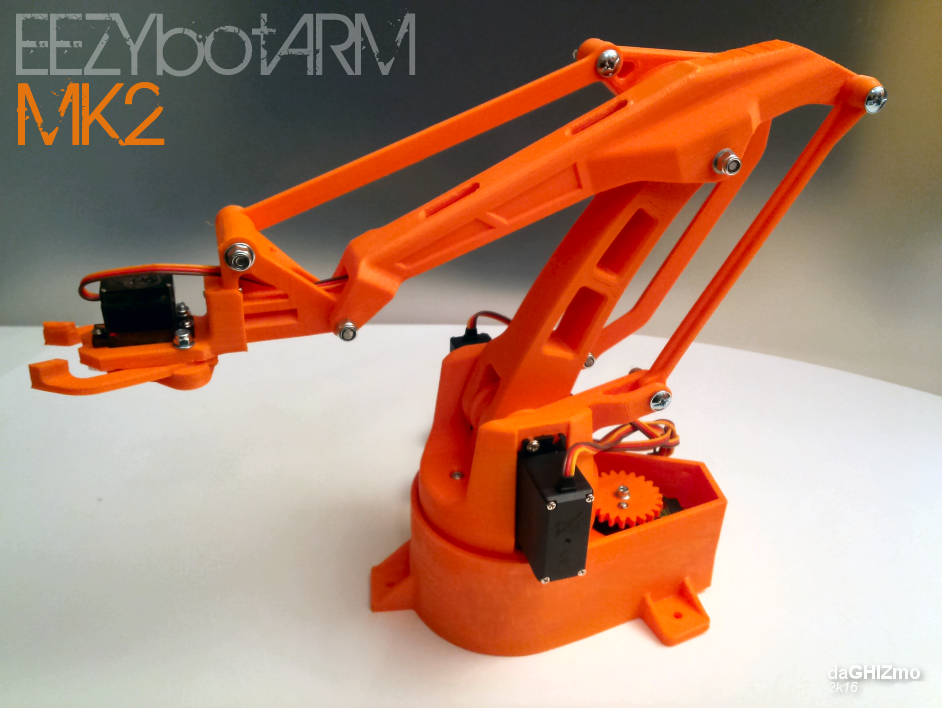
\includegraphics[width=0.8\linewidth]{image/rameno.png} 
			
		\end{figure}
		
		\vspace{0.02 \textheight}
		\begin{table}[h!]
			\begin{tabular}{ll}
				\textbf{Autor:} & \jmenoAutora\\ 
				\textbf{Obor:} & \kodOboru { } \obor\\
				\textbf{} & \zamereni\\
				\textbf{Třída:} & \trida\\
				\textbf{Školní rok:} & \skolniRok\\
			\end{tabular}
			
		\end{table}		
	}
	
\cleardoublepage %% Zalomení dvojstránky
	
%% Stránka obsahující poděkování a prohlášení
%%%%%%%%%%%%%%%%%%%%%%%%%%%%%%%%%%%%%%%%%%%%%%%%%%%%%%%%

%% Poděkování - nepovinné
%%%%%%%%%%%%%%%%%%%%%%%%%%%%
	
	\noindent{\large{\bfseries{Poděkování}\\}}
	\noindent Chci poděkovat Pánu učiteli Godovskému za poskytnutí veškerého hardweru a také konzultací během celé práci.
	
	\vspace*{0.7\textheight} %% Vertikální mezeru je možné upravit

%% Prohlášení - povinné
%%%%%%%%%%%%%%%%%%%%%%%%%%%%
	\noindent{\large{\bfseries{Prohlášení}\\}}  %% uprav si koncovky podle toho na jaký rod se cítíš, vypadá to pak lépe :) 
	\noindent{Prohlašuji, že jsem závěrečnou práci vypracovala samostatně a uvedla veškeré použité 
		informační zdroje.\\}
	\noindent{Souhlasím, aby tato studijní práce byla použita k výukovým a prezentačním účelům na Střední průmyslové a umělecké škole v Opavě, Praskova 399/8.}
	\vfill
	\noindent{V Opavě \datumOdevzdani\\}
	\noindent
	\begin{minipage}{\linewidth}
		\hspace{9.5cm} 
		\begin{tabular}{@{}p{6cm}@{}}
			\dotfill \\
			Podpis autora
		\end{tabular}
	\end{minipage}
	
	\cleardoublepage %% Zalomení dvojstránky

%% Stránka obsahující abstrakt (anotaci)
%%%%%%%%%%%%%%%%%%%%%%%%%%%%%%%%%%%%%%%%%%%%%%%%%%%%%%%%	

%% Abstrakt v češtině
%%%%%%%%%%%%%%%%%%%%%%%%%%%%
	\noindent{\Large{\bfseries{Abstrakt }\\}}
	\noindent 
	Výsledkem projektu je funkčí pohyblivé rameno, které zvláda chytnout kuličku z konce stavebnice a posune ji na začátek a také za dobře odvedenou práci se uklonit. Ovládáne je gesty které jsou snímány kamerou notebooku. Hlavním aspektem projektu je kontrola jednotlivých serv ramene pomocí gest. Kód který umožní zobrazovat  gesta je psaný v Pythonu, a holá pohyblivost ramene je obstarána Arduinem které využívá C++. 
	
	
	\vspace{18pt}
	
	\noindent{\large{\bfseries{Klíčová slova}}}
	
	\noindent poghyblivé rameno, gesta, Python, C++ \dots 
	
	\vspace{18pt}

%% Abstrakt v angličtině
%%%%%%%%%%%%%%%%%%%%%%%%%%%%	
	\noindent{\Large{\bfseries{Abstract}}}
	
	\noindent Write your abstract here! \lipsum[1] %% přepiš!!
	
	\vspace{18pt}
	
	\noindent{\large{\bfseries{Keywords}}}
	
	\noindent Template, \LaTeX, High school proffessional activity, \dots 
	
	\clearpage %% Zalomení stránky

%% Stránka s generovaným obsahem
%%%%%%%%%%%%%%%%%%%%%%%%%%%%%%%%%%%%%%%	
	
	\tableofcontents %% Vygeneruje tabulku s obsahem

	\pagenumbering{arabic} %% Nastavení způsobu číslování stránek (alternativy roman | Roman)
	\setcounter{page}{1} %% Nastavení počitadla stránek

%% Stránka s úvodem - povinná část
%%%%%%%%%%%%%%%%%%%%%%%%%%%%%%%%%%%%%%%		
	\chapter*{Úvod}

	\addcontentsline{toc}{chapter}{Úvod}
	

Tahle dokumentace vysvětluje celkovou funkčnost mého projektu. Kdyý jsme byli seznámení s tím, že čtvrtý ročník musíme zakončit ročnikovým projektem, byla jsem už rozhodnutá, že se můj projekt bude zabývat spíše Hardwarem. Po dlouhém a náročném pátrání a s pomocí pana Godovského jsem si pro svůj projekt nakonec vybrala robotické rameno. Bohužel samotné ovládání mě zavedlo primárně do Softwaru.

Rameno je ovládáné předvolenými gesty snímanými z kamery notebooku. Byl také nápad kompletně ovládat rameno způsobem, že rameno kopíruje pohyb ruky. Ale k tomu bylo potřeba dokoupit Pohyblivý senzor Kinect pro Xbox. To je ale celkem finančně náročné, tudíž od toho jsem odstoupila.	

Cílem projektu bylo zprovoznit pohyb ramene celkem jednoduchým ale také efektivním způsobem. Diky tomu jsem si skvěle procvičila Python a C++. Motivoval mě ten pocit že to rameno rozpohýbuji. 

Hned v první kapitole naleznete  všechny potřebné součástky k sestavení samotného ramene. To jsem ale nesestavovala já, tudíž se budu věnovat spíš softwaru. Je to doprovázené krátkou teorii o využitých technologiích. Nakonec také samozřejmě nebudou chybět odkazy ne všechny využité zdroje. 
%Tipy k psaní úvodu
%Je povinný, nadpis neměňte, rozsah - max. 1 strana. 
%Tato část práce obsahuje: 
%* náhled do řešené problematiky, zdůvodnění volby problematiky, 
%* předem definované cíle práce, 
%* motivaci pro další čtení textu včetně stručného uvedení obsahu následujících kapitol 


\chapter{Princip fungování projektu}
\begin{figure}[h]
	Tady se nachází strukturovaný náčrt, jak funguje celý projekt.
	A to tak že kamera snímá určité gesto. Kód s využitím knihoven obraz převádí na potřebné hodnoty které rozpozná rameno. Potom se pošlou do Arduina	a ono ve své řadě je dá na určité piny aby serva rozpoznala co mají dělat.
	\centering
	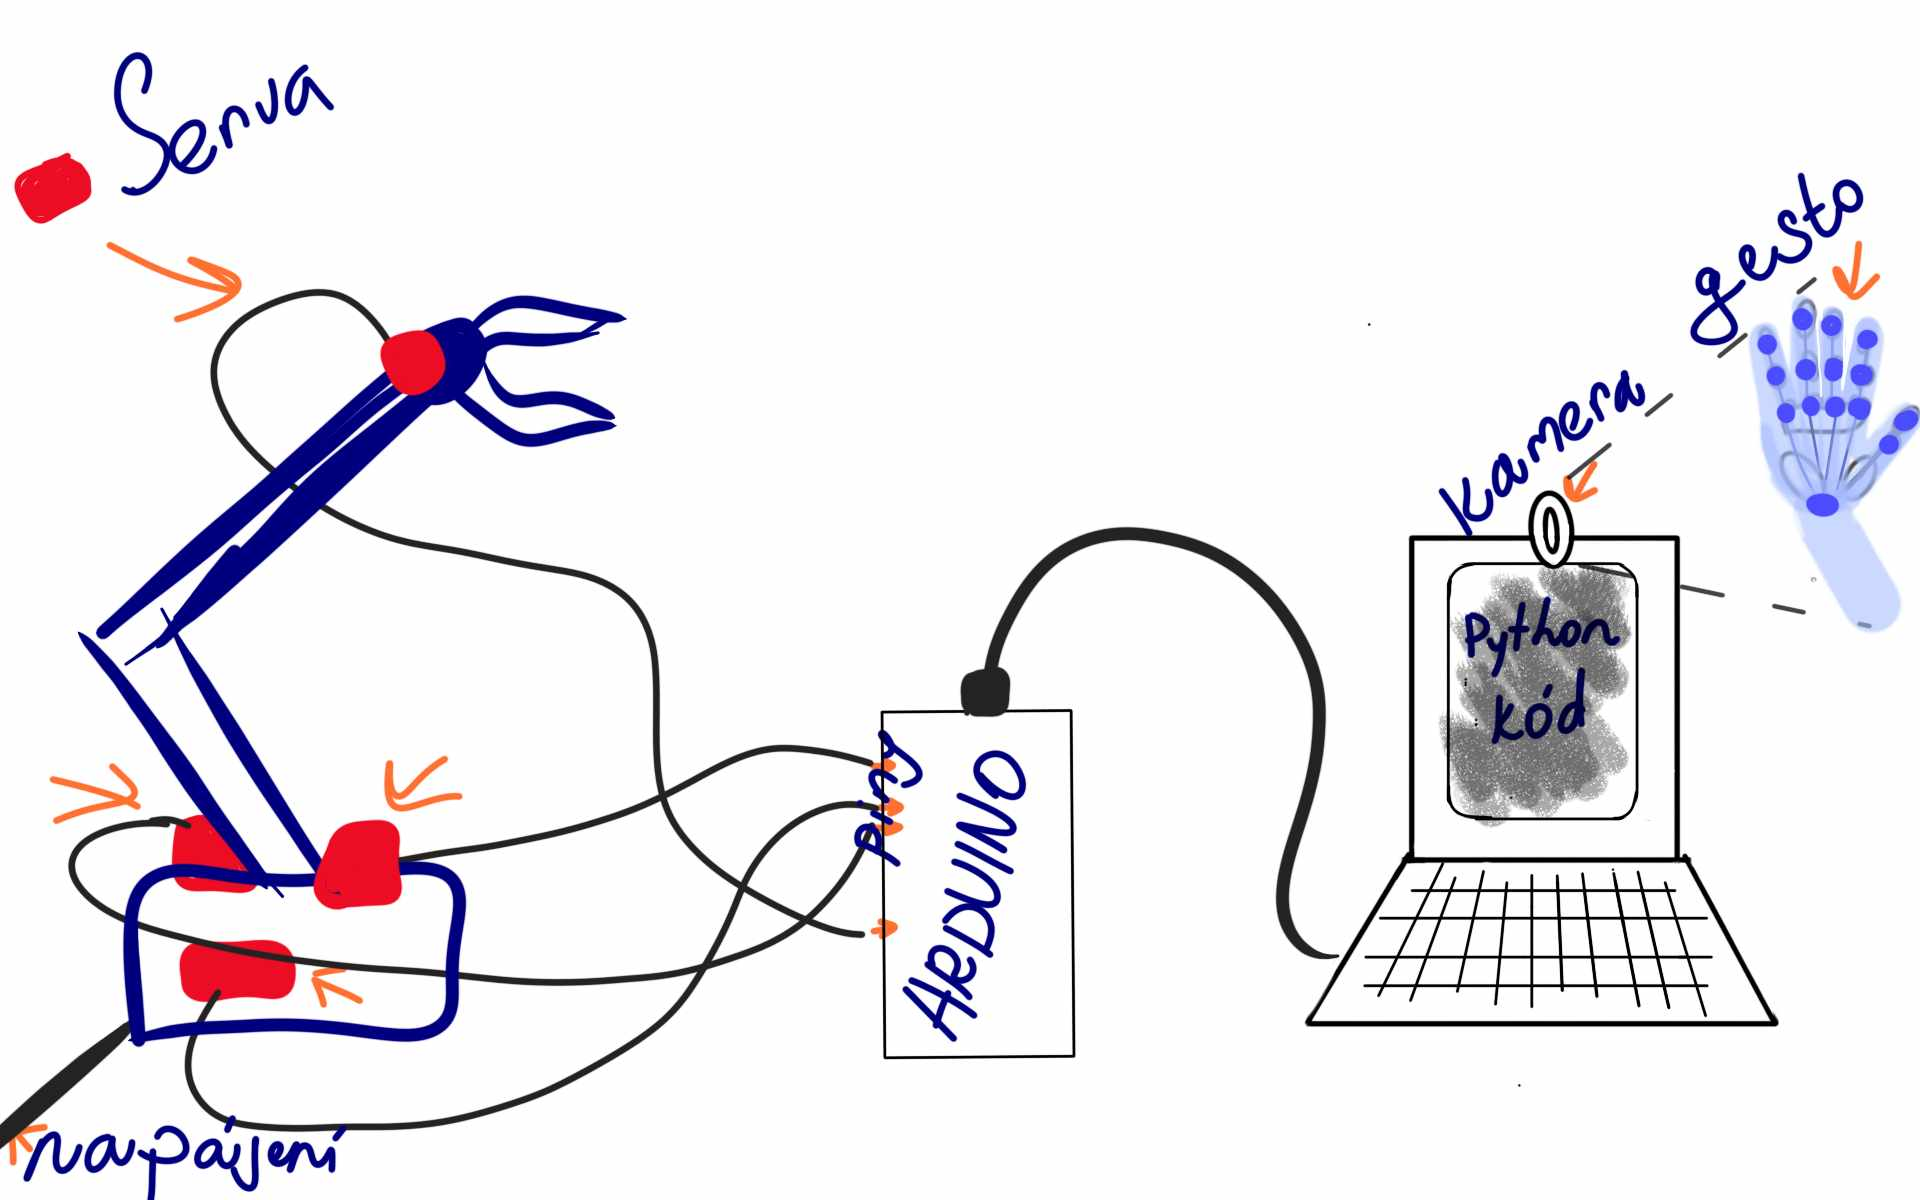
\includegraphics[width=0.9\linewidth]{image/princip.jpg} 
	
	
	\caption{Princip fungování projektu.} %% popisek obrázku, nezapomeň na citace!
	\label{fig:princip} %% označení až budeš chtít na obrázek odkazovat
\end{figure}


\chapter{Hardware}
	\section{Netištěné součástky}
Jelikož jsem to rameno nesestavovala tak nemam možnost popisovat postup, ale tady je výčet potřebných součástek 

\begin{itemize}
	\item	 3 - 955 nebo 946 servo
	\item 	1 - SG90 SERVO
	\item 	1 - Samojistná matice M6
	\item 	1 - Šroub M6x25
	\item 	2 - Samojistné matice M3
	\item 	2 - Šrouby M3 x 20
	\item 	1 - Šroub M3 x 10 se šestihrannou hlavou
	\item 	9 - Samojistné matice M4
	\item 	1 - Šroub M4 x 40
	\item 	1 - Šroub M4 x 30
	\item 	5 - Šroub M4 x 20
	\item 	1 - Závitová tyč M4 x 60mm
	\item 	1 - Závitová tyč M4 x 32 mm
	\item 	25 - Kulové koule o průměru 6 mm
	\item 	Ložisko 1 - 606zz
	\item 	Některé podložky M4
\end{itemize}


Návod na samotné sestavení ramene naleznete na \href{https://www.instructables.com/EEZYbotARM-Mk2-3D-Printed-Robot/}{tomhle odkazu} 
\newpage 


\subsection{Arduino nano 328}
\subsubsection{popis}

Arduino napomáha rozhýbat samotný hardwere. Napsaný kód, který popíšu v další kapitole nahrajeme pomocí USB kabelu do něj a diky správnému zapojení ramene vše skvěle funguje.


	\begin{figure}[h]
	
	\centering
	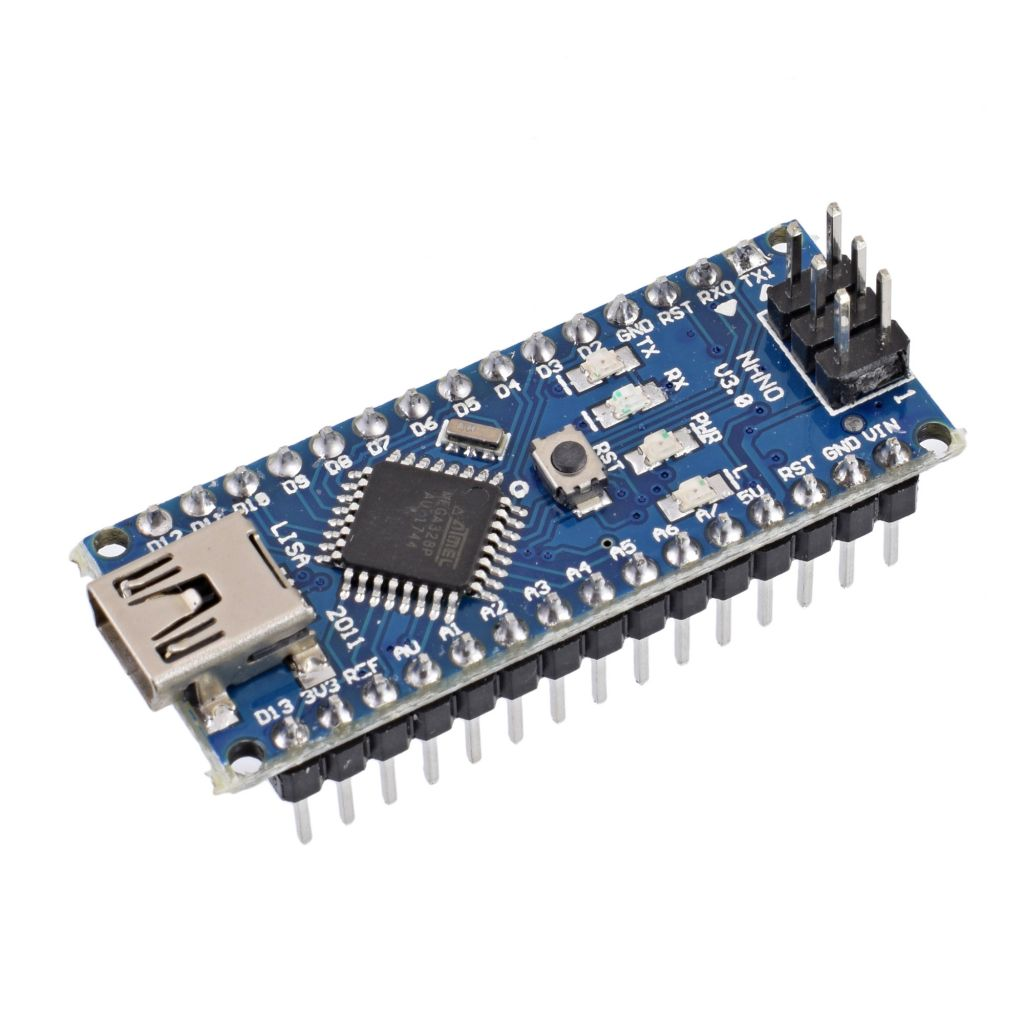
\includegraphics[width=0.6\linewidth]{image/arduino.jpg} 
	
	\caption{Arduino nano 328 } %% popisek obrázku, nezapomeň na citace!
	\label{fig:Arduino} %% označení až budeš chtít na obrázek odkazovat
\end{figure}

\newpage 

\subsection{Servo }
\subsubsection{popis}
	Tohle rameno obsahuje tři velké Serva a jedno malé.Každý
	z nich má také tři výstupy, a to: kabel určený na nějaký port, mínus a plus. 
	\\
	To nejmenší se nacházi v kleštičkách 
\begin{figure}[h]
	
	\centering
	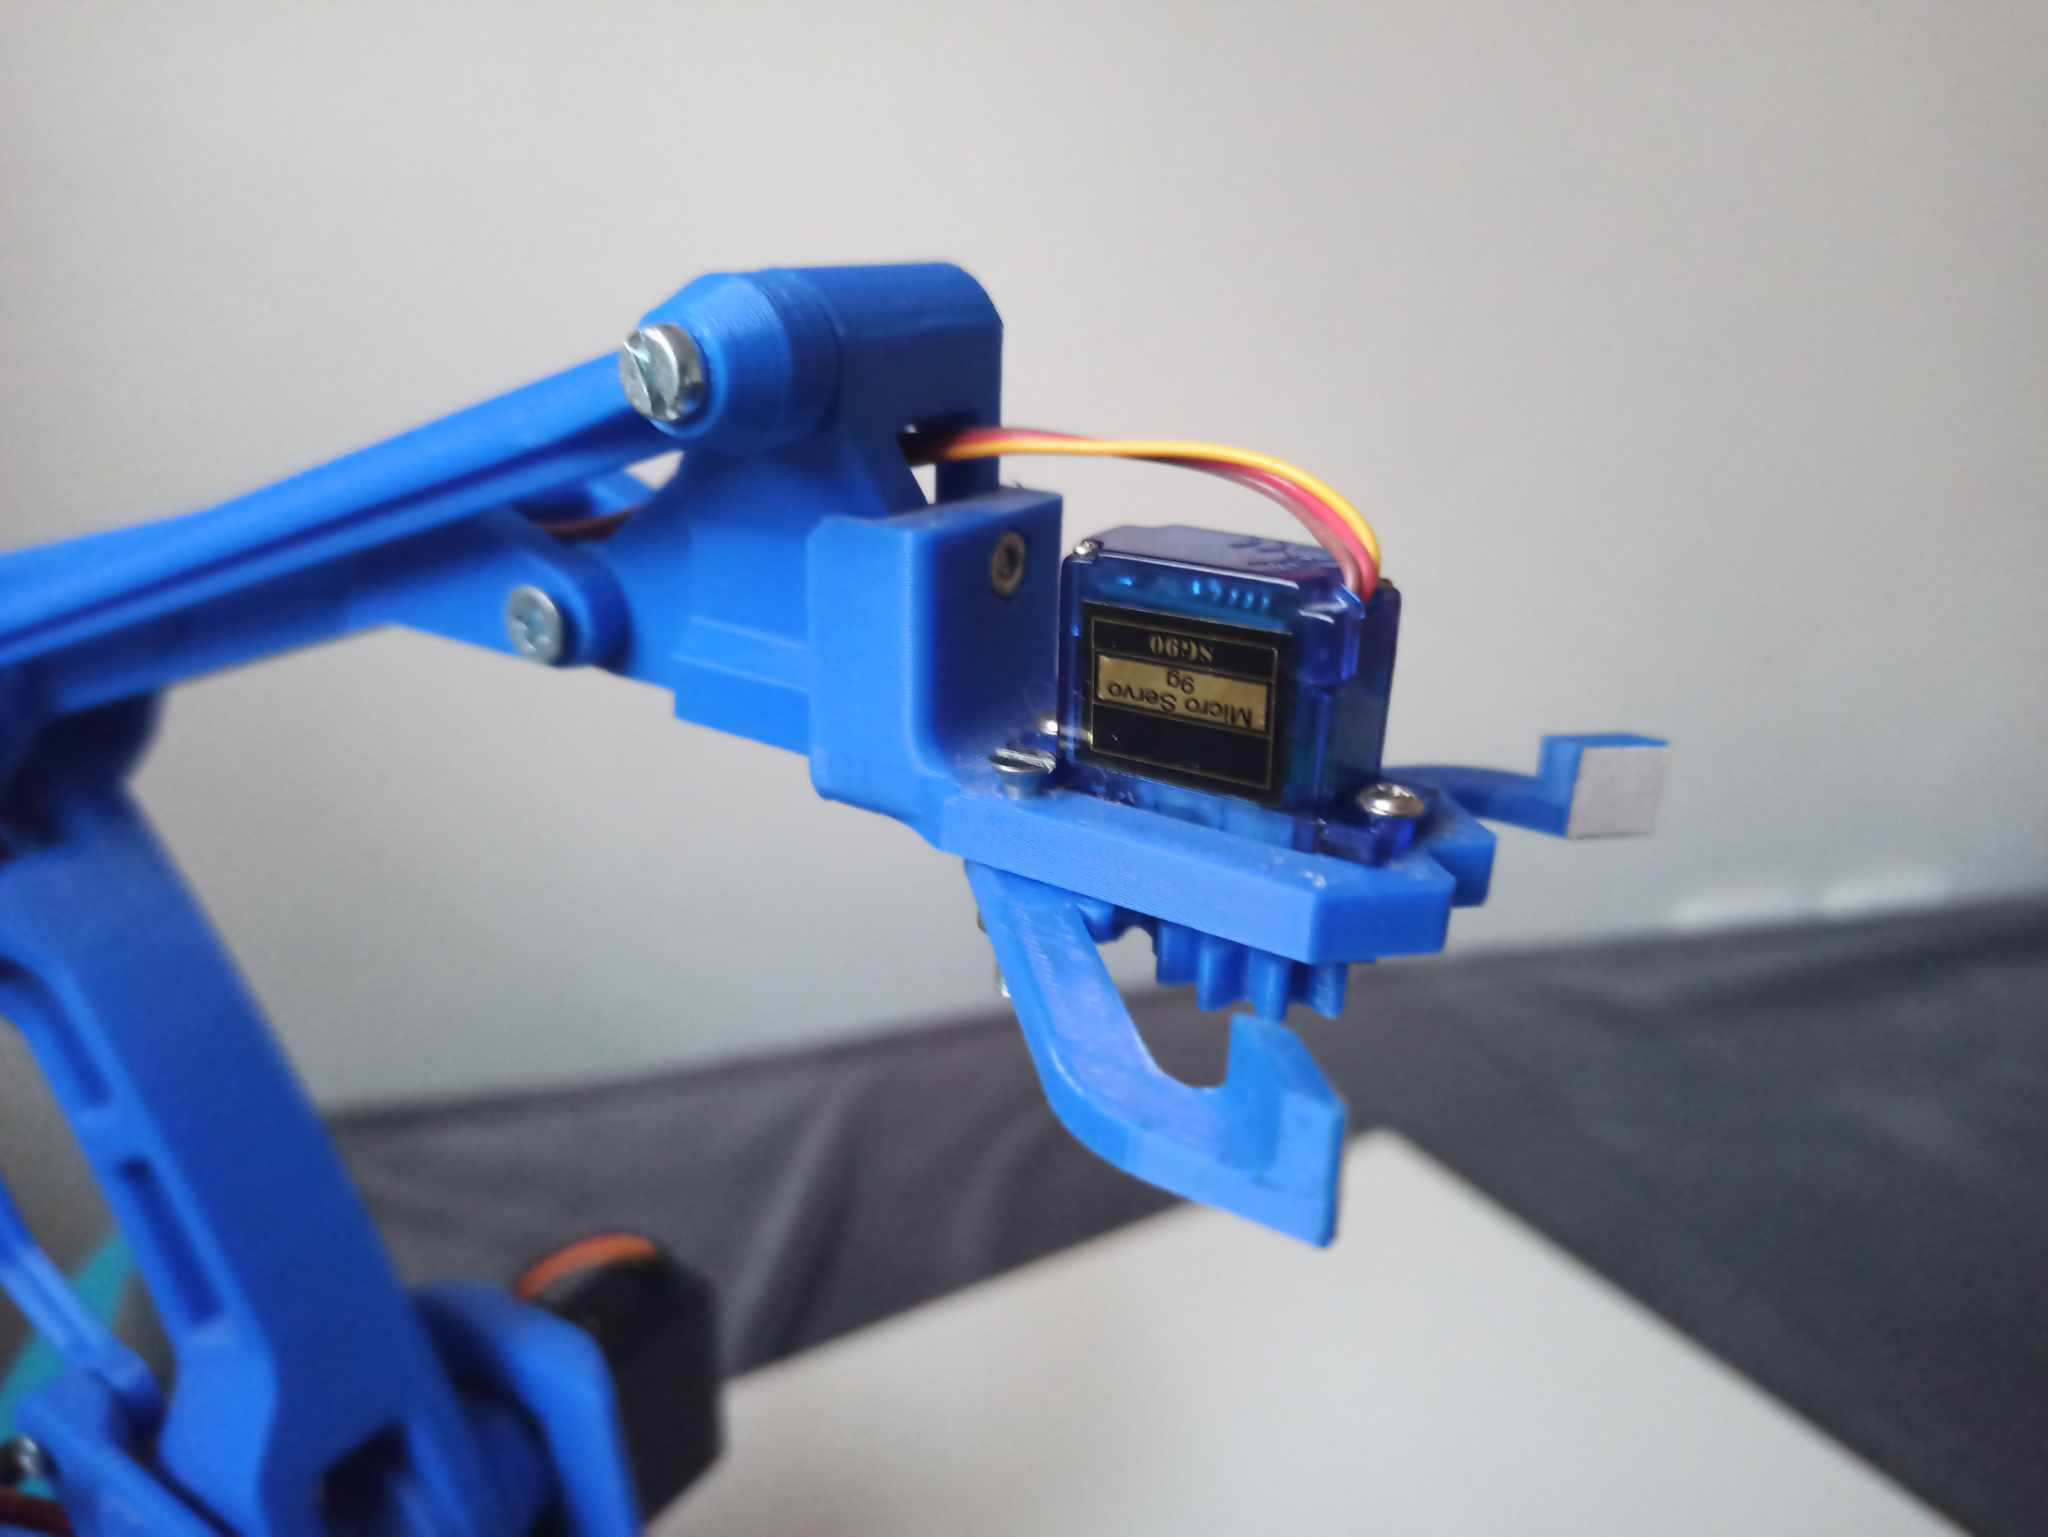
\includegraphics[width=0.5\linewidth]{image/kleste.jpg} 
	
	\caption{Servo nacházejíci se v kleštich ramene\cite{servo-kleste}.} %% popisek obrázku, nezapomeň na citace!
	\label{fig:Servo-kleste} %% označení až budeš chtít na obrázek odkazovat
\end{figure}

	Zbylé tři se zabývají rotací a pohyby nahoru-dolů, dopředu-dozadu

\begin{figure}[h]
	
	\centering
	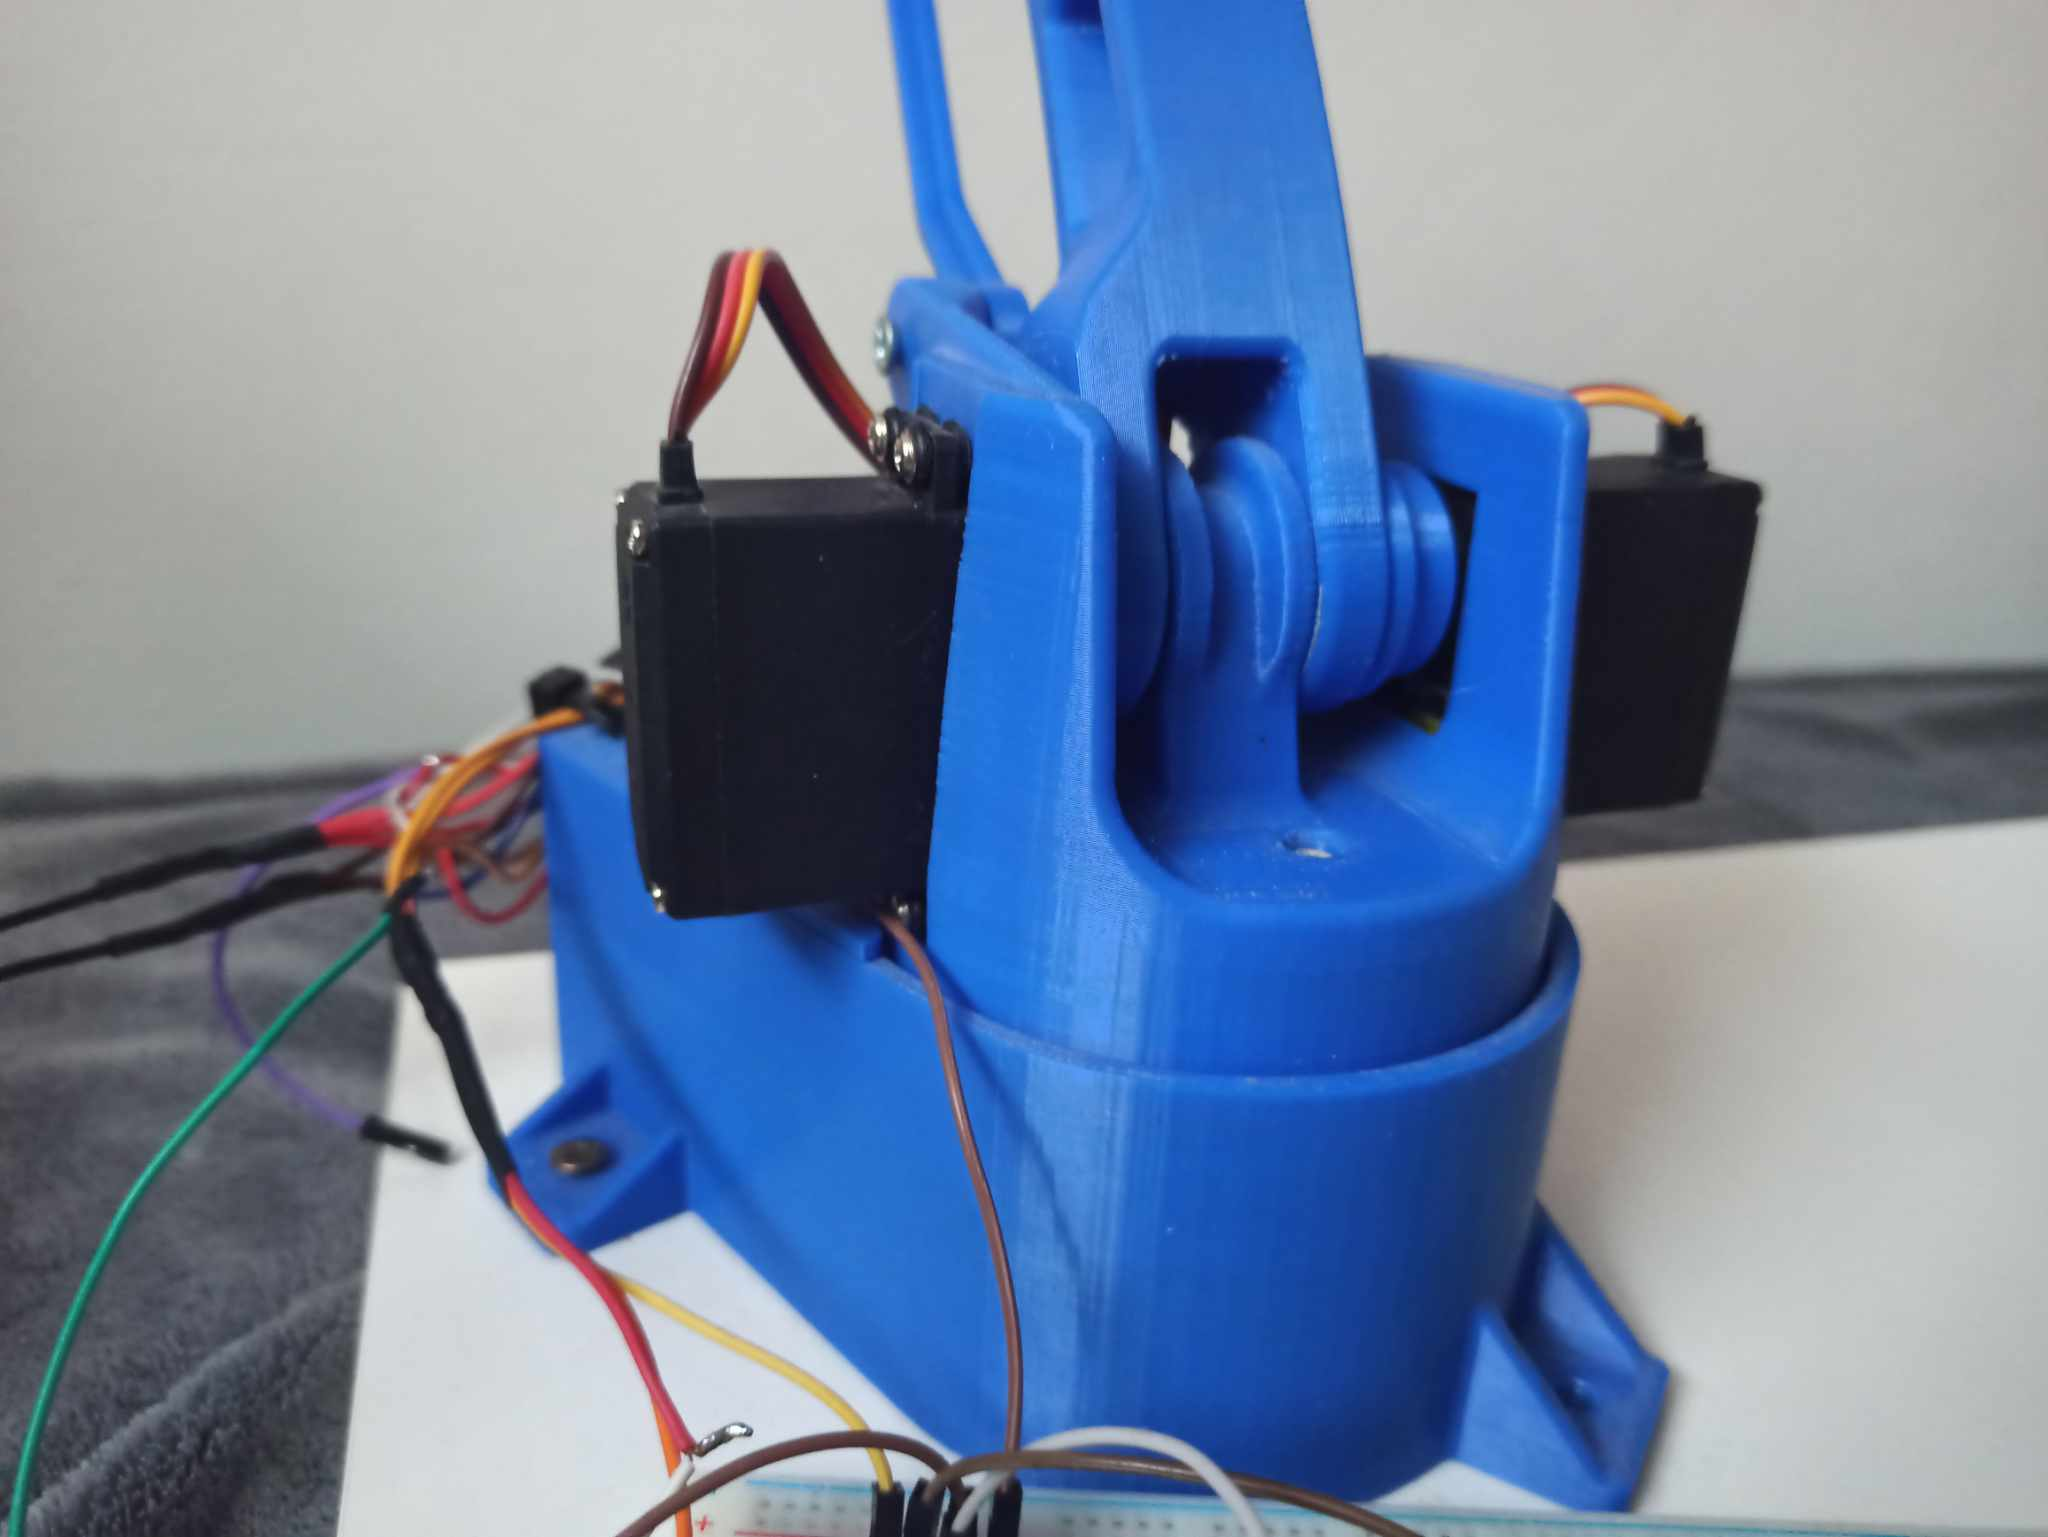
\includegraphics[width=0.5\linewidth]{image/serva.jpg} 
	
	\caption{Serva v těle ramene.} %% popisek obrázku, nezapomeň na citace!
	\label{fig:Serva} %% označení až budeš chtít na obrázek odkazovat
\end{figure}

\newpage

\subsection{Obvod}

\begin{figure}[h]
	
	\centering
	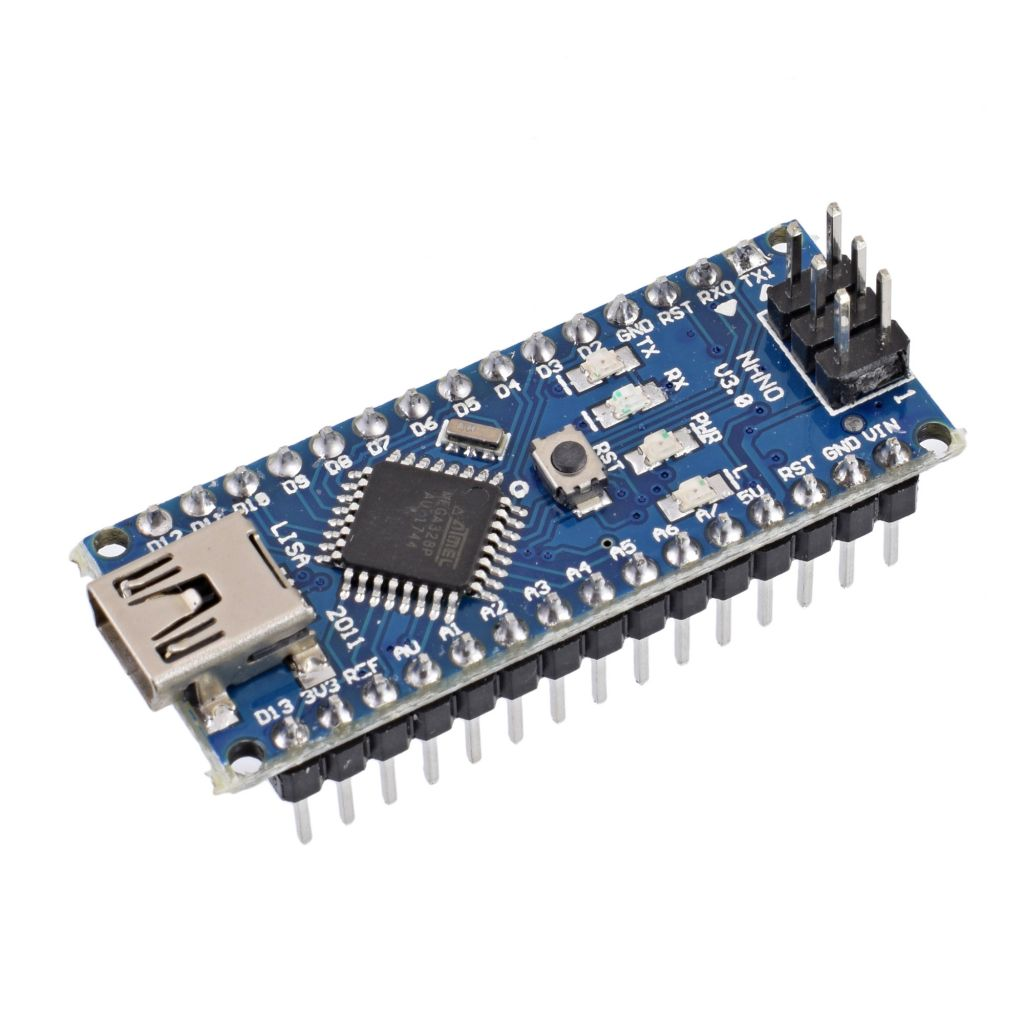
\includegraphics[width=0.9\linewidth]{image/arduino.jpg} 
	
	
	\caption{Zapojení ramene.} %% popisek obrázku, nezapomeň na citace!
	\label{fig:obvod} %% označení až budeš chtít na obrázek odkazovat
\end{figure}

\newpage




\chapter{Software}

\section{Získání gest}
Začneme importem knihoven, a to \textbf{OpenCV}  \textbf{math} a \textbf{mediapipe 0.10.8}  

\subsubsection{Knihovna OpenCV}
OpenCV je multiplatformní svobodná knihovna pro práci s obrazem.

 Samotná knihovna je z velké části napsána v C++, ale poskytuje Python wrapper, díky kterému ji můžeme používat i v Pythonu. 
 OpenCV se používá pro zpracování obrazu z kamer, rozpoznání psaného textu nebo obličejů..
Tuto knihovnu jsem využila na celkové zpracování obrazu z kamery mého notebooku


\begin{lstlisting}[style=Python, caption={Obraz, a jeho převedení do správného formátu}]
cap = cv2.VideoCapture(0)
...
image = cap.read()
imageRGB = cv2.cvtColor(image, cv2.COLOR_BGR2RGB)
results = hands.process(imageRGB)
\end{lstlisting}

Převede snímáný obraz do formátu RGB, který potřebujem pro vykreslení pixelů ve správném pořadí.

\subsubsection{Knihovna MediaPipe}

Tahle knihovna se zaměřuje na detekci lidských části těla.
Já využila pro svůj projekt pouze detekci dlaní.
Pro detekci potřebuje mít orientační body ruky. Model ručního orientačního bodu dokáže předpovědět 21 přesných souřadnic umístění každého orientačního bodu na ruce.

\begin{figure}[h]
	
	\centering
	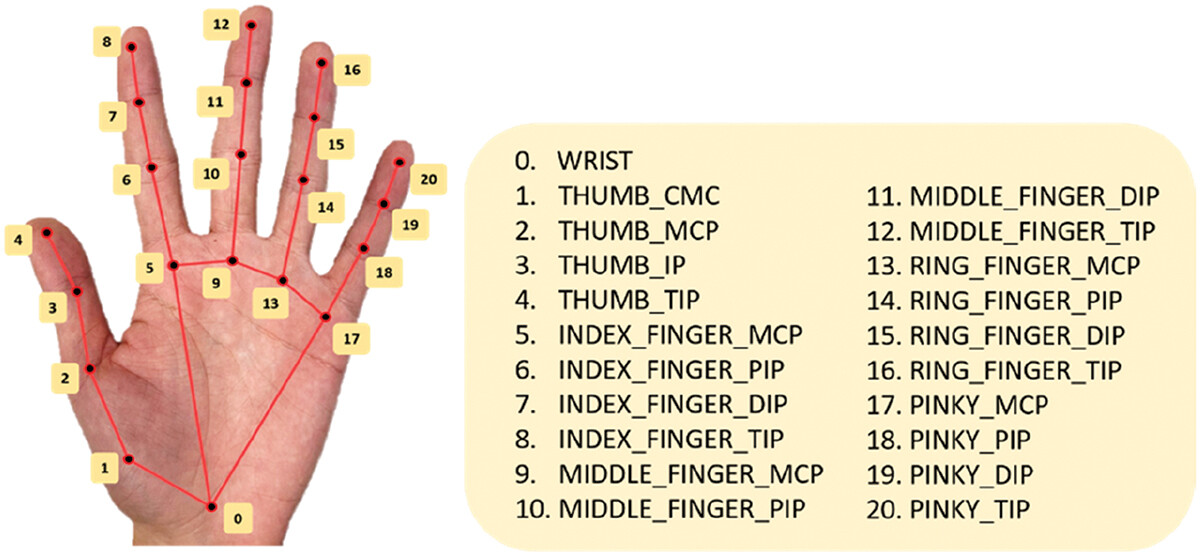
\includegraphics[width=0.8\linewidth]{image/orientacniBody.jpg} 
	
	
	\caption{Orientacni body dlaně.} %% popisek obrázku, nezapomeň na citace!
	\label{fig:obvod} %% označení až budeš chtít na obrázek odkazovat
\end{figure}

\subsubsection{Knihovna math}

Ve spolupráci se zvyše zmíněnou knihovnou mi poskytla souřadnice jednotlivých kloubu, pro přesné zachycení ruky. 
Další výpočty provedla také při zachycení vzdálenosti prstů potřebné k rozhýbání kleštiček

\begin{figure}[h]
	
	\centering
	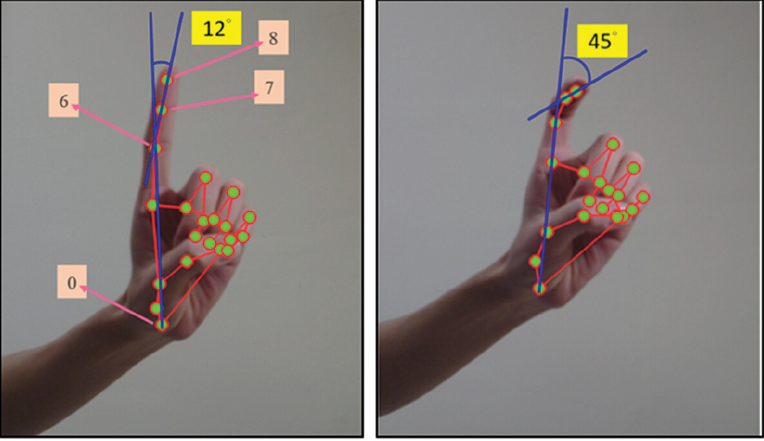
\includegraphics[width=0.4\linewidth]{image/prikladGesta.PNG} 
	
	
	\caption{Použití úhlu v gestech.} %% popisek obrázku, nezapomeň na citace!
	\label{fig:uhlyVGestech} %% označení až budeš chtít na obrázek odkazovat
\end{figure}
\begin{figure}[h]
	
	\centering
	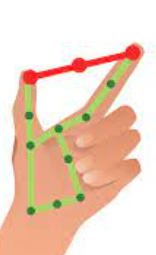
\includegraphics[width=0.2\linewidth]{image/vzdalenost.PNG} 
	
	
	\caption{Použití měření vzdálenosti v gestech.} %% popisek obrázku, nezapomeň na citace!
	\label{fig:vzdalenost} %% označení až budeš chtít na obrázek odkazovat
\end{figure}



\newpage

\section{Ověření funkčnostní ramene}
Než jsem mohla začit se sprovozněním ramene dle myšlenky, jsem musela ověřit jejích funkčnost a taky zjistit jak se vlastně jednotlivá část hýbe.
Proto jsem použila jednoduhý kód. Připojením pokaždé jednoho drátku do desky s arduinem jsem se postupně dozvěděla zaprve jaký drátek zodpovídá za co a také i jak se hybou. Byl tam jeden zadrhel a to to že serva stávkovaly, když jsem posílala ty krajní hodnoty(0,180) po úpravě intervalu ve funkci, se všechno srovnalo.

\begin{lstlisting}[style=Python, caption={Ukázka kódu k ověření funkčnosti}]
#include <Servo.h>

Servo myservo;  

int pos = 0;    
void setup() {
	myservo.attach(9);  
}

void loop() {
	for (pos = 2; pos <= 160; pos += 1) { 
		myservo.write(pos);             
		delay(15);                      
	}
	for (pos = 160; pos >= 2; pos -= 1) {
		myservo.write(pos);            
		delay(15);                       
	}
}
\end{lstlisting}

\newpage

\section{Práce s Arduinem}

První věc, kterou musíme vzít v úvahu, je, že nezbytně potřebujeme mít na svém počítači program Python a také PySerial. Většinu kódu v Pythonu se dá sehnat na internetu a odkazy na ty stránky nalezenete níže v použité literatuře. 
Takže se jdeme přesunout k popisu.
Pro kód v C++ je na zčátek potřeba inicializovat veškere potřebné hodnoty.
např:

\begin{lstlisting}[style=Python, caption={Inicializace potřebných hodnot}]
const int min= 2;  // minimalní hodnota rozmezí pro vzdálenost
const int max = 160; // maximalní hodnota rozmezí pro vvzdálenost

bool end;
int data = 0;
int serialData =0;
bool changeMode;
int mode;
const int servoPose = 6; //kolik stavu má rameno
const int servoCount = 4; // počet serv

Servo servo[4]; // pole pro serva 
const byte servoPins [] = {2,3,4,5}; //piny pro serva
\end{lstlisting}


\begin{itemize}
	\item Jelikož potřebujeme pro pohyb kleští hodnoty mezi 0 - 180, musíme posílanou vzdálenost přemapovat a k tomu využívám proměnné min a max které nám značí rozmezí posílaných hodnot
	\item changeMode je pro přehazování mezi snímáním počtu prstu nebo vzdálenosti mezi prsty
	
\begin{figure}[h]
	
	\centering
	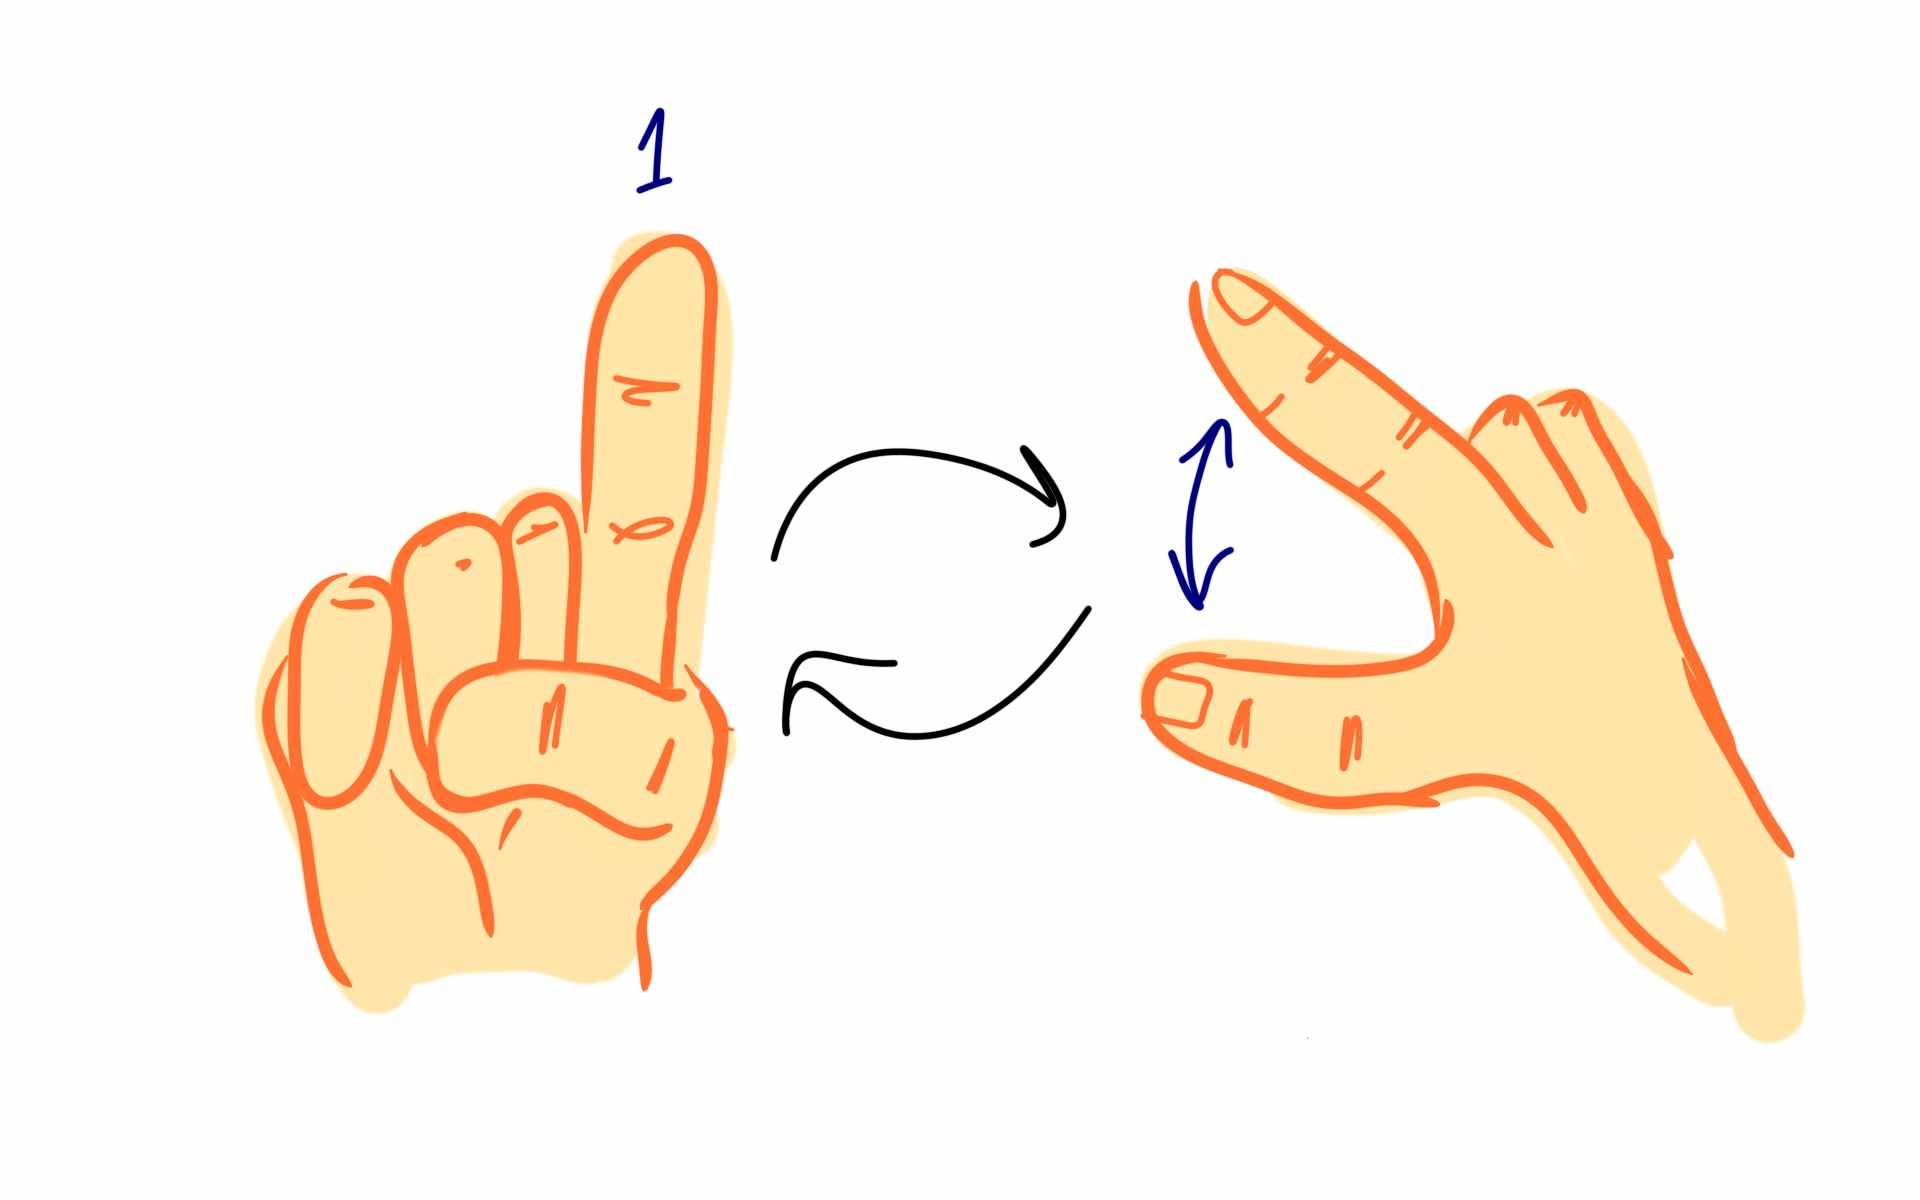
\includegraphics[width=0.3\linewidth]{image/mody.jpg} 
	
	
	\caption{Dvá módy pro kontrolu ramene.} %% popisek obrázku, nezapomeň na citace!
	\label{fig:uhlyVGestech} %% označení až budeš chtít na obrázek odkazovat
\end{figure}
\item   V proměnné servoPos je uložen počet všech stavu ve kterých se moje rameno může nacházet.
\item Jelikož obsahuje 4 serva, tak jsem pro ně vytvořila pole. A každé potřebuje svůj pin k tomu je proměnná servoPins.
	
\end{itemize}



\begin{lstlisting}[style=Python, caption={Podmínka pro přepínání módu}]
if(j == (servoMoves[data][0] -1)) {
	if(data == 0 || data == 1) {
		changeMode = true;
		mode = data;
	}
\end{lstlisting}

\begin{itemize}
		\item Tahle jednoduchá podmínka je vytvořena pro kontrolu, kde se zrovna nachází rameno. A když se nachází nahoře nebo dole, tak se přepné mód pro měření vzdálenosti. Ať se může chytnout nebo pustit kulička.

	
\end{itemize}
	
\begin{lstlisting}[style=Python, caption={Dvourozměrné pole na potřebné hodnoty}]
	 int servoValues [13] [3] = {
		{20,50,20},  //puvodni stav 
		{170,80,45}, //dole sběr kuličky cast1
		{123,113,45}, //dolu sběr kuličky cast2
		...
		{123,130,133},  //uklona cast2
	};
		\end{lstlisting}
		
\begin{itemize}
	\item Dále máme dvourozměrné pole pro hodnoty pro serva. jsou vždy v jednom řádku jen tři, protože pro ovádání serva v kleštích jsou potřeba jiné hodnoty.
			
	\end{itemize}
	
\begin{lstlisting}[style=Python, caption={Další pole pro několik hodnot }]
	int servoMoves [servoPose] [3] = {
		{2,1,500}, //dolu ke kulice 1
		{2,3,500}, //nahoru ke kulice 2
		{5,5,700}, //ne  3
	...
	};	
	\end{lstlisting}
	
	\begin{itemize}
		\item Další pole se skládá z několika různých hodnot. A to na prvním místě počet opakování pohybů, na druhém místě se nachází pořadí hodnot serv z předešlého pole.Poslední hodnota je pro delay.
		
	\end{itemize}

\begin{lstlisting}[style=Python, caption={Funkce na rozpohybocání ramene}]	
	void move(int data) {
		int cycle = 0;
		for(int j = 0 ; j < servoMoves[data][0];j++) {
			for(int i = 1; i < servoCount;i++) servo[i].write(servoValues[
											(servoMoves[data][1])+cycle][i -1]);
			cycle++;
			if(cycle > 1) cycle=0;
			if(j == (servoMoves[data][0] -1)) {
				if(data == 0 || data == 1) {
					changeMode = true;
					mode = data;
				}
				end = true;
				Serial.begin(9600);
			}
			delay(servoMoves[data][2]);
		}
	}
	
	\end{lstlisting}
	
	\begin{itemize}
		\item Jedna z nejpodstatnějších funkcí. Je pro rozpohybování ramene.
		Jakmile se načte jedna hodnota, funkce se posune v cyklu o jedno políčko dál v servoValues, a tak než dojde na konec. Potom se zkontroluje zda data jsou 0 nebo 1 pro pochopení že se rameno nacházi v pozici u  kuličky. Tehdy se změní changeMode a přepne se na měření vzdálenosti mezi prsty.
		
	\end{itemize}
	
	
	
	
	
	
	
	\chapter*{Závěr}
	\addcontentsline{toc}{chapter}{Závěr}
	
	Cílem samotné práce bylo rozpohybovat rameno a udělat si jasno jak fungují knihovny. Ve finální verzi rameno je schopno uchytit kuličku a přenést ji z konce na začátek. Všechno to je vyřešeno pomocí Pythonu a C++. Využití tohohle projektu může být různé. Například v továrnách, ve skladech, v nanochirurgii nebo jako vzdělávácí hračky. Začátečný cíl se mi podařilo splnit a rameno funguje tak, jak jsem si původně představovala při zahájení vývoje. I přes můj výkon kód přece jen není napsán nejoptimálněji a věřím, že by mohl být mnohem lépe zkonstruován, což do budoucná bych mohla opravit. Také později bych se chtěla víc zaměřit na knihovnu OpenCV a prozkoumat další její funkce. 

	
	%% literatura
	\renewcommand\bibname{Seznam použitých zdrojů}
	\begin{thebibliography}{99}
		\addcontentsline{toc}{chapter}{Seznam použitých zrdojů}
		\bibitem{sablonaSOC}{Základní informace o gestech} [Online].  2023 CEMI MBA Studies s.r.o. [cit. 2020-08-24]. Dostupné z: \url{https://www.cemi.cz/blog/neverbalni-komunikace-co-prozradi-gesta}
		
		\bibitem{LaTeXprirucka} {Typy gest v běžném životě} [online]. 1998 [cit. 2020-08-24]. Dostupné z: \url{https://orangeacademy.cz/clanky/rec-tela/}
		
		\bibitem{wikibooksLaTeX} Řeč tela a znakový jazyk, 2023, Slůně - svět jazyků, s.r.o. Dostupné z: \url{https://www.slune.cz/aktualita/znakovy-jazyk/}
		
		\bibitem{wikibooksLaTeX} Knihovna math v pythonu Copyright © 2023 itnetwork.cz.
	 \url{https://www.itnetwork.cz/python/zaklady/python-tutorial-knihovny-math-a-random}
	 	\bibitem{wikibooksLaTeX} Knihovna opencv v pythonu Copyright © 2023 itnetwork.cz.
	 \url{https://www.python-programator.cz/clanky/python-pro-zpracovani-obrazu-opencv}
	 \bibitem{wikibooksLaTeX} Komunikace s arduinem  © 2023 Arduino
	 \url{https://projecthub.arduino.cc/ansh2919/serial-communication-between-python-and-arduino-663756}
	 \bibitem{wikibooksLaTeX}Komunikace s arduinem 2 Copyright © 2023 Circuit Digest. All rights reserved.
	 \url{https://circuitdigest.com/microcontroller-projects/arduino-python-tutorial}
	  \bibitem{© 2023 Arduino}Zkouška funkčnosti 
	 \url{https://docs.arduino.cc/learn/electronics/servo-motors}
	  \bibitem{wikibooksLaTeX}Zkouška funkčnosti 
	 \url{https://problemsolvingwithpython.com/11-Python-and-External-Hardware/11.03-Controlling-an-LED/}
	 
	 
	 
		
		
		
	
	\end{thebibliography}
	
	%% obrázky 
	\listoffigures
	

	
	\appendix %% začínají přílohy
	
	\titleformat{\chapter}[block]{\scshape\bfseries\LARGE}{Příloha \thechapter}{10pt}{\vspace{0pt}}[\vspace{-22pt}] %% nastavení nadpisu u příloh
	
	

	
	
\end{document}